\documentclass{beamer}

\author[D. Abercrombie]{
  Daniel Abercrombie \\
  Guillelmo Gomez-Ceballos \\
  Benedikt Maier
}

\title{\bf \sffamily Rough Regression}
\date{\today}

\usecolortheme{dove}

\usepackage[absolute,overlay]{textpos}
\usefonttheme{serif}
\usepackage{appendixnumberbeamer}
\usepackage{isotope}
\usepackage{hyperref}
\usepackage[english]{babel}
\usepackage{amsmath}
\setbeamerfont{frametitle}{size=\Large,series=\bf\sffamily}
\setbeamertemplate{frametitle}[default][center]
\usepackage{siunitx}
\usepackage{tabularx}
\usepackage{makecell}
\usepackage{comment}

\setbeamertemplate{navigation symbols}{}
\usepackage{graphicx}
\usepackage{color}
\setbeamertemplate{footline}[text line]{\parbox{1.083\linewidth}{\footnotesize \hfill \insertshortauthor \hfill \insertpagenumber /\inserttotalframenumber}}
\setbeamertemplate{headline}[text line]{\parbox{1.083\linewidth}{\footnotesize \hspace{-0.083\linewidth} \textcolor{blue}{\sffamily \insertsection \hfill \insertsubsection}}}

\IfFileExists{/Users/dabercro/GradSchool/Presentations/MIT-logo.pdf}
             {\logo{\includegraphics[height=0.5cm]{/Users/dabercro/GradSchool/Presentations/MIT-logo.pdf}}}
             {\logo{\includegraphics[height=0.5cm]{/home/dabercro/MIT-logo.pdf}}}

\usepackage{changepage}

\newcommand{\beginbackup}{
  \newcounter{framenumbervorappendix}
  \setcounter{framenumbervorappendix}{\value{framenumber}}
}
\newcommand{\backupend}{
  \addtocounter{framenumbervorappendix}{-\value{framenumber}}
  \addtocounter{framenumber}{\value{framenumbervorappendix}}
}

\graphicspath{{figs/}}

\newcommand{\link}[2]{\href{#2}{\textcolor{blue}{\underline{#1}}}}
\newcommand{\clink}[2]{\link{#1}{http://t3serv001.mit.edu/~dabercro/redir/?k=#2}}}

\newcommand{\twofigs}[4]{
  \begin{columns}
    \begin{column}{0.5\linewidth}
      \centering
      \textcolor{blue}{#1} \\
      \includegraphics[width=\linewidth]{#2}
    \end{column}
    \begin{column}{0.5\linewidth}
      \centering
      \textcolor{blue}{#3} \\
      \includegraphics[width=\linewidth]{#4}
    \end{column}
  \end{columns}
}

\newcommand{\fourfigs}[8]{
  \begin{columns}
    \begin{column}{0.3\linewidth}
      \centering
      \textcolor{blue}{#1} \\
      \includegraphics[width=\linewidth]{#2} \\
      \textcolor{blue}{#3} \\
      \includegraphics[width=\linewidth]{#4}
    \end{column}
    \begin{column}{0.3\linewidth}
      \centering
      \textcolor{blue}{#5} \\
      \includegraphics[width=\linewidth]{#6} \\
      \textcolor{blue}{#7} \\
      \includegraphics[width=\linewidth]{#8}
    \end{column}
  \end{columns}
}

\newcommand{\ttbar}{\ensuremath{t\bar{t}}}
\newcommand{\bbbar}{\ensuremath{b\bar{b}}}

\begin{document}

\begin{frame}
  \titlepage
\end{frame}

\begin{frame}
  \frametitle{Introduction}

  \begin{itemize}
  \item Trained on di-lepton $tt$, but single lepton samples ready
  \item Training using kinematics of
    \begin{itemize}
    \item Jet
    \item Leptons
    \item EM, Charged, Neutral contributions
    \item $\Delta R$ rings
    \item PUPPI components (charged, neutral)
    \end{itemize}
  \item Deep CSV and QGL
  \item Also including event info such as pileup and number of jets
  \item Still throwing together this morning
  \item Using native TensorFlow APIs to allow future flexibility
  \item Will also use TensorFlow for classification
  \end{itemize}

\end{frame}

\begin{frame}
  \frametitle{Model -- Combined}
  \centering
  \includegraphics[width=0.9\linewidth]{full.png}
\end{frame}

\begin{frame}
  \frametitle{Model -- DNN}
  \centering
  \includegraphics[width=0.5\linewidth]{dnn.png}
\end{frame}

\begin{frame}
  \frametitle{Model -- Linear}
  \centering
  \includegraphics[width=0.5\linewidth]{linear.png}
\end{frame}

\begin{frame}
  \frametitle{Loss Function}
  \centering
  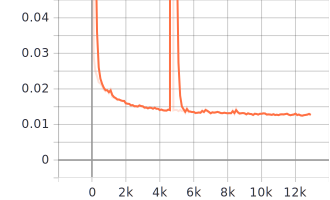
\includegraphics[width=0.7\linewidth]{loss.png}

  Huber loss function \textcolor{red}{$\delta = 1.0$}, will be fixed

\end{frame}

\begin{frame}
  \frametitle{Fraction of Zeros}
  \centering
  \includegraphics[width=0.7\linewidth]{frac.png}
\end{frame}

\begin{frame}
  \frametitle{Regression Results}
  \centering
  \includegraphics[width=0.7\linewidth]{190417_breg_new/hbb_m_tf_v10__hbb_m_tf_v9__hbb_m_tf_v2__hbb_m.pdf}

  DNN, \textcolor{red}{linear}, \textcolor{green}{combined}, \textcolor{blue}{untrained}

\end{frame}

\begin{frame}
  \frametitle{Regression Results -- with $\Delta \eta, \Delta \phi$}
  \centering
  \includegraphics[width=0.7\linewidth]{190417_breg_old/hbb_m_tf_v10__hbb_m_tf_v9__hbb_m_tf_v2__hbb_m.pdf}

  DNN, \textcolor{red}{linear}, \textcolor{green}{combined}, \textcolor{blue}{untrained}

\end{frame}

\begin{comment}
\beginbackup

\begin{frame}
  \frametitle{Backup Slides}
\end{frame}

\begin{frame}
   \frametitle{\small 190611/plot\_time\_60000\_wide}
   \centering
   \includegraphics[width=0.6\linewidth]{190611/plot_time_60000_wide.pdf}
\end{frame}

\begin{frame}
   \frametitle{\small 190611/plot\_time\_wide}
   \centering
   \includegraphics[width=0.6\linewidth]{190611/plot_time_wide.pdf}
\end{frame}

\begin{frame}
   \frametitle{\small 190611/plot\_time\_120000\_compare}
   \centering
   \includegraphics[width=0.6\linewidth]{190611/plot_time_120000_compare.pdf}
\end{frame}

\begin{frame}
   \frametitle{\small 190611/plot\_time\_60000\_compare}
   \centering
   \includegraphics[width=0.6\linewidth]{190611/plot_time_60000_compare.pdf}
\end{frame}

\begin{frame}
   \frametitle{\small 190611/plot\_time\_80000\_compare}
   \centering
   \includegraphics[width=0.6\linewidth]{190611/plot_time_80000_compare.pdf}
\end{frame}

\begin{frame}
   \frametitle{\small 190611/plot\_time\_120000\_narrow}
   \centering
   \includegraphics[width=0.6\linewidth]{190611/plot_time_120000_narrow.pdf}
\end{frame}

\begin{frame}
   \frametitle{\small 190611/plot\_time\_40000\_narrow}
   \centering
   \includegraphics[width=0.6\linewidth]{190611/plot_time_40000_narrow.pdf}
\end{frame}

\begin{frame}
   \frametitle{\small 190611/plot\_time\_160000\_narrow}
   \centering
   \includegraphics[width=0.6\linewidth]{190611/plot_time_160000_narrow.pdf}
\end{frame}

\begin{frame}
   \frametitle{\small 190611/plot\_time\_60000\_narrow}
   \centering
   \includegraphics[width=0.6\linewidth]{190611/plot_time_60000_narrow.pdf}
\end{frame}

\begin{frame}
   \frametitle{\small 190611/plot\_time\_80000\_narrow}
   \centering
   \includegraphics[width=0.6\linewidth]{190611/plot_time_80000_narrow.pdf}
\end{frame}

\begin{frame}
   \frametitle{\small 190611/plot\_time\_narrow}
   \centering
   \includegraphics[width=0.6\linewidth]{190611/plot_time_narrow.pdf}
\end{frame}



\backupend
\end{comment}

\end{document}
